\section{Results}

In the present study, we investigated the differences in gaze-based planning strategies dependent on task, tool familiarity, and handle orientation. Here, we investigated two anticipatory gaze-based strategies 3 seconds before action initiation; the odds of fixations in favor of the tool effector and the dynamic changes in the eccentricity of the fixations relative to the center of the tool. We further compared the oculomotor differences in two experiments that had the same experimental conditions but differed in action affordance of the interaction method in VR. 


\begin{figure}[ht]
    \centering
    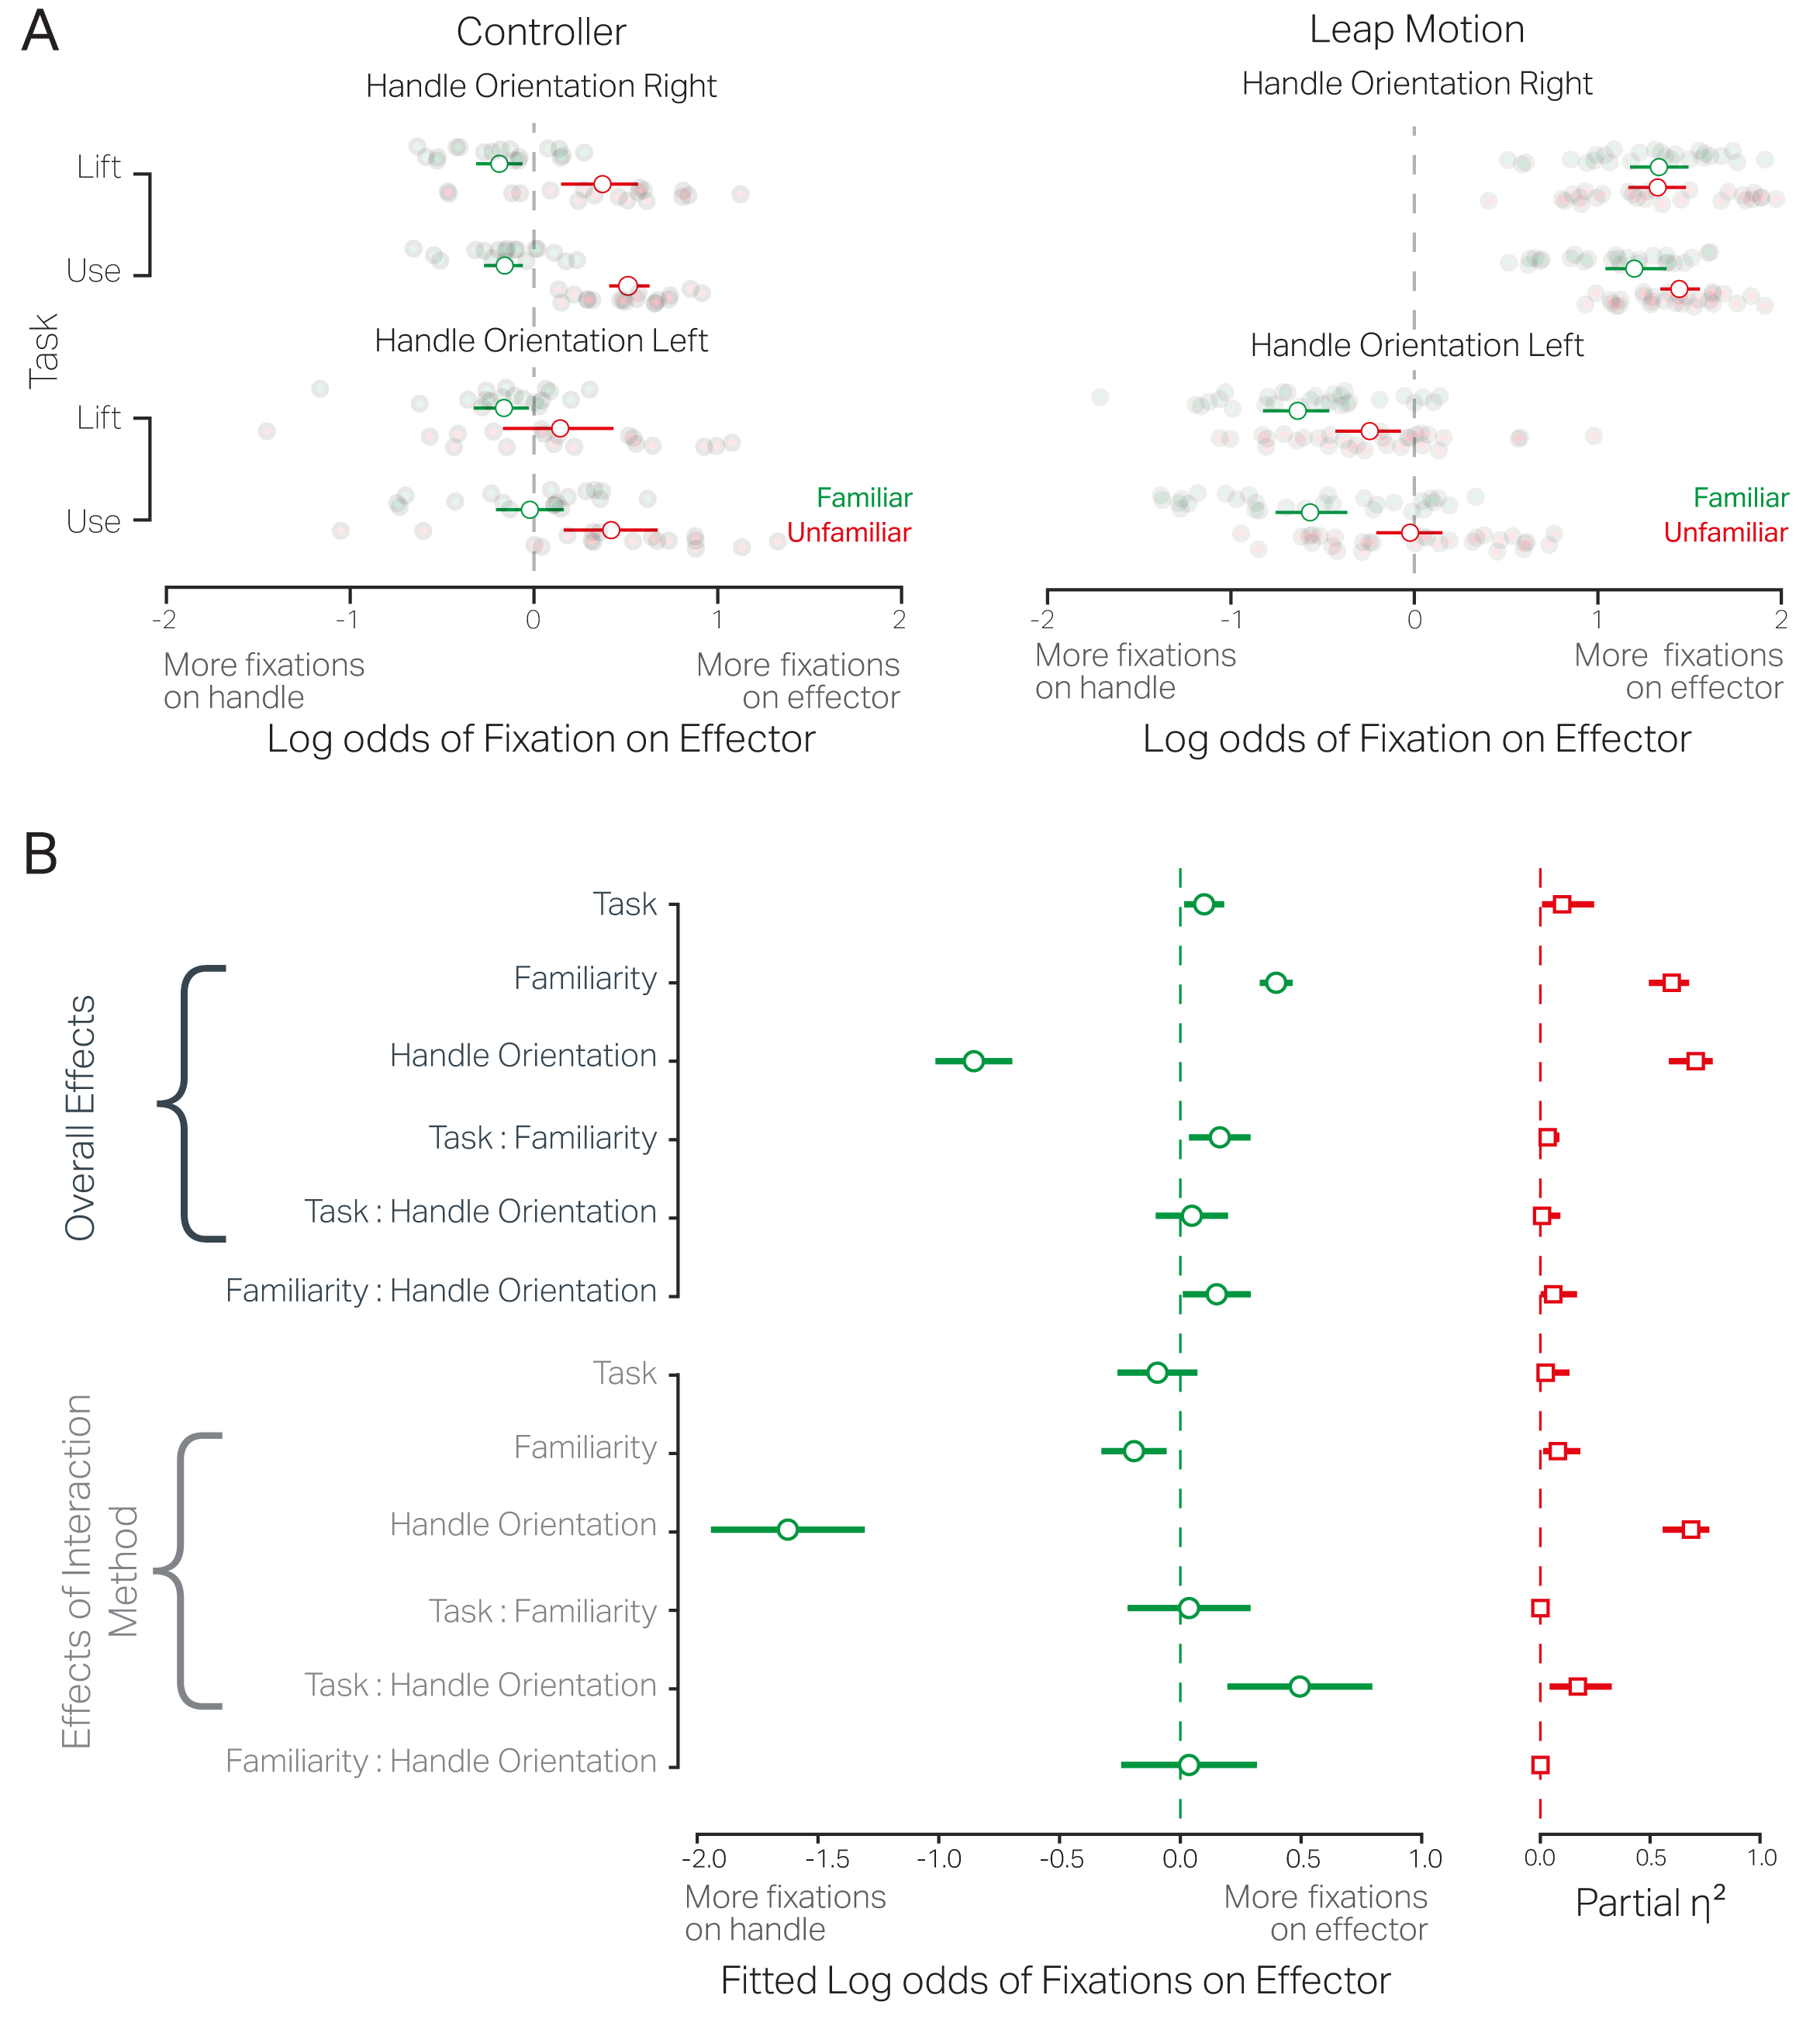
\includegraphics[width=0.85\linewidth]{source/figures/result/full_model_cdata_coefs.png} \\
    \caption[]{Effect of task, tool familiarity, handle orientation, interaction method on log-odds of fixations . \textbf{A)} \textbf{top-left:} shows the log-odds of fixation on effector vs. handle in the controller study when the tool handle is oriented to the right. The log odds on fixations are higher on the effector for unfamiliar tools (red) than the familiar tools (green) for both the LIFT and the USE tasks. \textbf{Bottom-left:} log odds of fixation on effector when the tool handle is oriented to the left and is incongruent to the subjects’ handedness. The plot shows that the orientation of the tool does not significantly affect the log-odds fixation on the effector. \textbf{Top-right:} the log-odds of fixation on effector in the LeapMotion study when the tool handle is oriented to the right. The log odds of fixations on the effector are higher for unfamiliar tools (red) than the familiar tools (green) and the USE task. \textbf{Bottom-right:} log odds of fixation on effector when the tool handle is oriented to the left and is incongruent to the subjects’ handedness. The plot shows that the orientation of the tool results in significant log-odds of fixations over the handle in the LIFT task, while in the USE task and with unfamiliar tools (red) significantly more fixations were on the effector. \textbf{B.)} The regression coefficients (green) and their 95\%confidence and associated effect-size (red) from the fitted linear mixed model. The regression coefficients and 95\%confidence intervals that do not include null are significant. 
}
    \label{figure:log_odds}
\end{figure}

First, we compared the log-odds of fixations in favor of the tool effector across the three conditions: task, tool familiarity, and handle orientation in the 3s period when the subjects studied the tool. Figure 3A shows the log-odds of the fixations on the tool effector for experiment-I (with VR Controllers) and experiment-II (with LeapMotion). In experiment-I (Figure \ref{figure:log_odds}A, left panel), subjects showed a mean log odds of 0.04 (95\%CI = [-0.04, 0.11]) for the LIFT task and for the USE task the mean log-odds were 0.17 (95\%CI = [0.08, 0.26]). For the FAMILIAR tools, the mean log-odds in favor of the tool effector were -0.14 (95\%CI = [-0.21, -0.07]) and for UNFAMILIAR 0.34 (95\%CI = [0.23, 0.45]). For the  RIGHT oriented tool handle, the mean log-odds were 0.14 (95\%CI = [0.06, 0.22]) and for the LEFT oriented tool handle, the mean log-odds were 0.08 (95\%CI = [-0.09, 0.26]). In experiment-II (Figure \ref{figure:log_odds}A, right panel), subjects showed a mean log odds of 0.16 (95\%CI = [-0.01, 0.31]) of fixations on the tool effector for the LIFT task and for the USE task the mean log-odds were 0.24 (95\%CI = [0.09, 0.38]). For the FAMILIAR tools, the mean log-odds in favor of the tool effector were 0.08 (95\%CI = [-0.06, 0.23]) and for UNFAMILIAR 0.30 (95\%CI = [0.15, 0.44]). For the RIGHT oriented tool handle, the mean log-odds were 1.31 (95\%CI = [1.21, 1.42]) and for the LEFT oriented tool handle, the mean log-odds were -0.32 (95\%CI = [-0.45, -0.19]). 

To statistically assess the significant differences between the experimental factors, we used linear mixed models. For the linear model, we used effect coding so the regression coefficients can be directly interpreted as main effects. Figure \ref{figure:log_odds}B shows the estimated regression coefficients and their associated effect size. Taking the experiment groups together, there was a main effect of factor task (USE - LIFT) $\beta$ = 0.1 (95\%CI = [0.02, 0.182], t(50.32)=2.35, p = 0.02, $\eta_p^2$ = 0.1, 90\%CI = [0.01, 0.24]) ). There was also significant main effect of familiarity (UNFAMILIAR - FAMILIAR ) $\beta$ = 0.40  (95\%CI = [0.33, 0.46], t(89.14)=11.52, p < 0.001, $\eta_p^2$ = 0.6, 90\%CI = [0.49, 0.68]). There was also a main effect of handle orientation (LEFT - RIGHT) $\beta$ = -0.85, (95\%CI = [-1.01, -0.70], t(45.75)=-10.52, p < 0.001, $\eta_p^2$ = 0.71, 90\%CI = [0.59, 0.78]). There was an overall a significant interaction of task and familiarity with $\beta$ = 0.16, 95\%CI = [0.04, 0.29], t(184.17) = 2.53, p = 0.01, $\eta_p^2$ = 0.03, 90\%CI = [0.0, 0.09]).  The was also a significant interaction of task and handle orientation $\beta$ = 0.15, 95\%CI = [0.01, 0.29], t(71.32) = 2.11, p = 0.04, $\eta_p^2$ = 0.06, 90\%CI = [0.0, 0.17]). The interaction of familiarity and orientation was not significant , $beta$ = 0.05, 95\%CI = [-0.1, 0.2], t(51.03) = 0.63, p = 0.53, $\eta_p^2$ = 0.01, 90\%CI = [0.0, 0.09]). In sum, irrespective of the interaction methods employed in the two experiments, there were significantly higher odds of fixations on effector in the USE task, for UNFAMILIAR tools. Moreover, there were significantly lower odds of fixations on the effector when the tool handles were oriented to the LEFT and in-congruent to the subjects' handedness.

The linear model showed the effects of the interaction method used in the two experiments. There was no significant difference between the experiments for the factor of task ($\beta$ = -0.09, 95\%CI = [-0.26, 0.07], t(50.32) = -1.12, p = 0.27, $\eta_p^2$ = 0.02, 90\%CI = [0.0, 0.13]). There was a significant difference in the effects of familiarity between the experiment groups ($\beta$ = -0.19, 95\%CI = [-0.33, -0.06], t(89.14) = -2.78, p = 0.01, $\eta_p^2$ = 0.08, 90\%CI = [0.01, 0.18]). There was a significant difference between the experimental groups for the factor handle orientation $\beta$ = -1.62 (95\%CI = [-1.94, -1.31], t(45.75) = -10.0, p = 0.0, $\eta_p^2$ = 0.69, 90\%CI = [0.56, 0.77]), where the LeapMotion experiment biased fixations towards the tool handle as compared to the controller experiment when the tool handle was oriented to the LEFT. There were no significant difference in the interaction of of task and familiarity between the experimental groups ($\beta$ = 0.04, 95\%CI = [-0.22, 0.29], t(184.17) = 0.28, p = 0.78, $\eta_p^2$ = 0.0, 90\%CI = [0.0, 0.02]). There was a significant difference between groups in the interaction effects of familiarity and handle orientation ($\beta$ = 0.5, 95\%CI = [0.2, 0.79], t(51.03) = 3.24, p = 0.0, $\eta_p^2$ = 0.17, 90\%CI = [0.04, 0.32]). There was no significant difference between groups for interaction between task and handle orientation ($\beta$ = 0.04, 95\%CI = [-0.24, 0.32], t(71.32) = 0.26, p = 0.8, $\eta_p^2$ = 0.0, 90\%CI = [0.0, 0.04]). In a nutshell, the largest difference between the experimental groups was seen when the tool handle was oriented to the LEFT and in-congruent to the subjects' handedness.


\begin{figure}[ht]
    \centering
    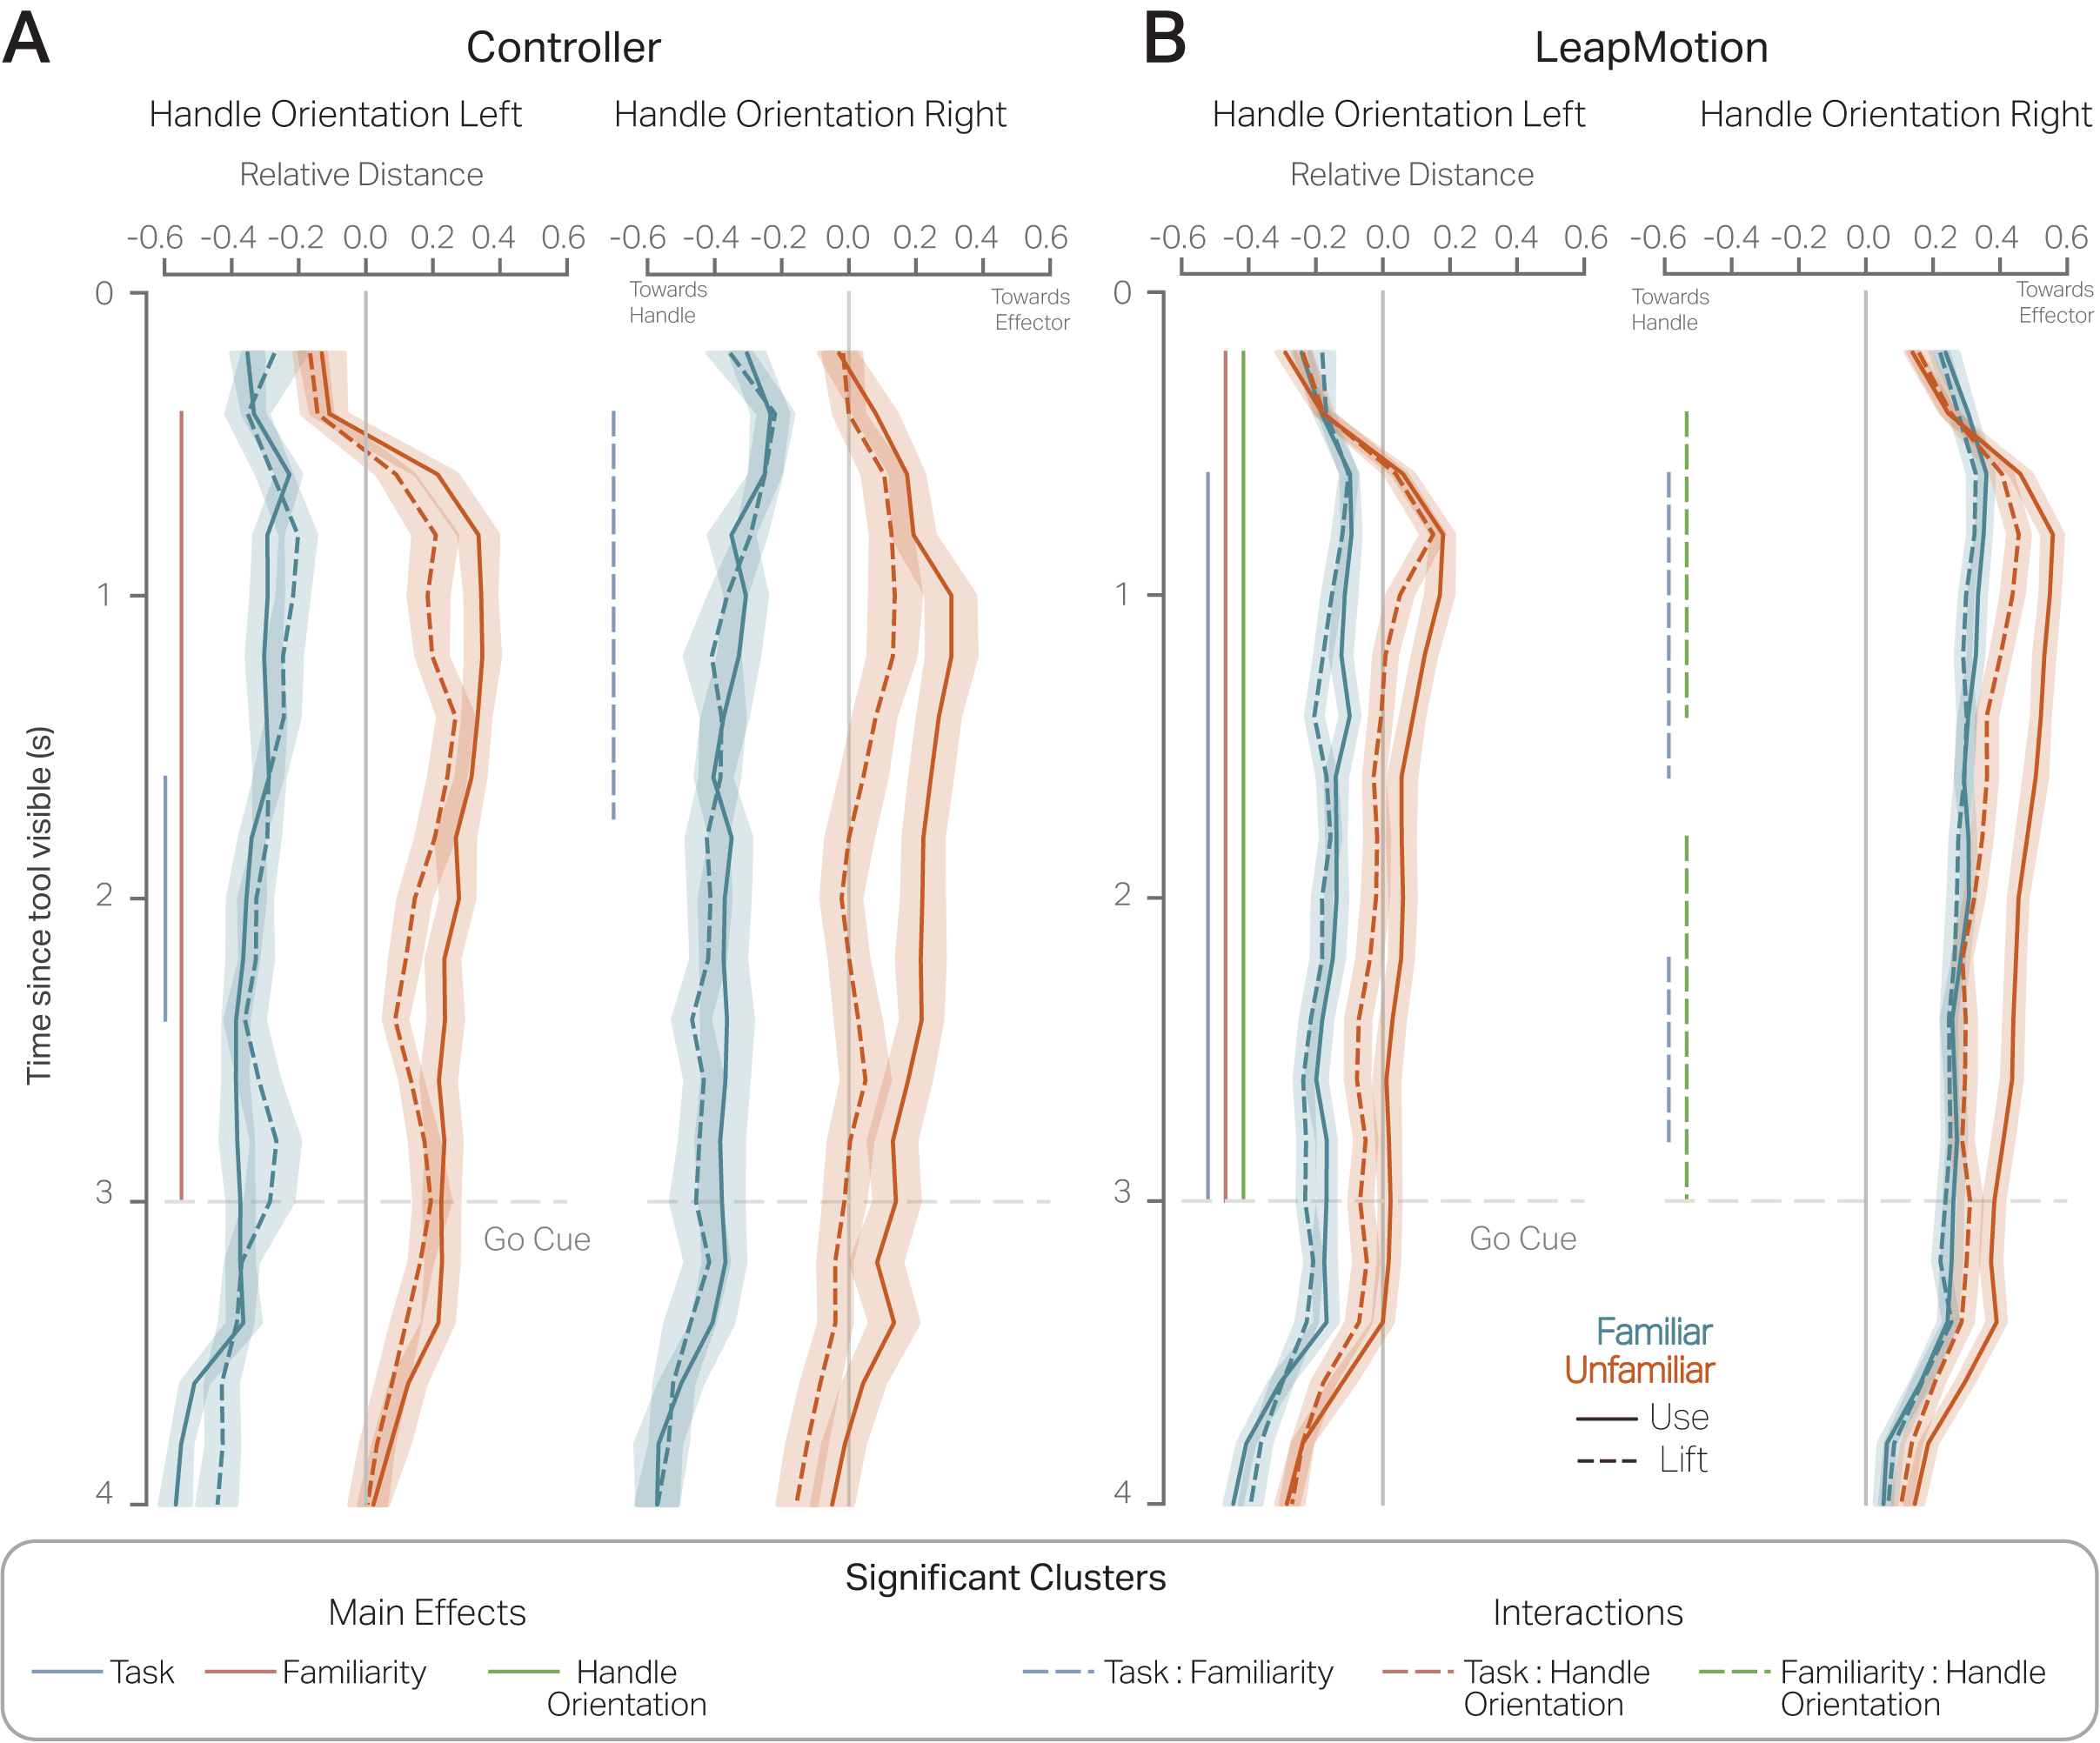
\includegraphics[width=0.9\linewidth]{source/figures/result/deviation_from_center_new.png} \\
    \caption[]{Eccentricity of fixations on the tool models. The negative values of the abscissa correspond to fixations towards the handle, the positive values refer to fixations towards the tool effector, and zero represents the center of the tool. The ordinate axis refers to the time elapsed since the tool is visible on the virtual table. The go cue is given to participants at 3s after which they can start interacting with the tool. The blue lines correspond to the FAMILIAR tool and red to the UNFAMILIAR tools. The error bars represent the standard error of the mean across subjects.  The vertical solid lines correspond to the significant time clusters for main effects and the vertical dashed lines to the interactions. \textbf{A} Eccentricity of fixations from the tool center in and the two handle orientations. \textbf{B.} Eccentricity of fixations from the tool center in experiment-II and the two handle orientations.
}
    \label{figure:dev_from_center}
\end{figure}

Next, we were interested in the effect of task, tool familiarity, and handle orientation on the eccentricity of the fixations on the tool before action initiation. We calculated the relative distance of fixations from the center of the tool in the 3s period when the subjects studied the tool. We used cluster permutation tests to evaluate the time periods where the experimental conditions elicited significant differences. As shown in Figure \ref{figure:dev_from_center}A, in experiment-I, the differences in task (USE - LIFT) were significant from 1.06s to 2.6s after tool presentation, p < 0.001. Differences in tool familiarity (UNFAMILIAR - FAMILIAR) were significant from 0.4s to 3s with a p-value <0.001. Moreover, the differences in the handle orientation (LEFT - RIGHT) were not significant. The interaction of task and familiarity were significant from 0.4s to 1.8s, p=0.02. In sum, while interacting with the VR controller, there were effects of use task and unfamiliar tools that biased the fixations towards the tool effector and the orientations of the tool handle did not affect this bias significantly.

Similarly, figure \ref{figure:dev_from_center}B shows the eccentricity of fixations from the center of the tool during the 3s period when the subjects studied the tool in experiment-II with LeapMotion as the interaction method. The differences in task were significant from 0.6s to 3s, p< 0.001. The differences in familiarity were significant from 0.2s to 3s, p < 0.001. Furthermore, the differences in handle orientation were significant from 0.2s to 3s, p < 0.001. There was a significant interaction of task and familiarity from 0.6s to 1.6s with p = 0.008 and from 2.2s to 2.8s, p = 0.03. There were also significant clusters in the interaction of tool familiarity and handle orientation from 0.4s to 1.4s with p = 0.007 and from 1.8s to 3s, p = 0.007. In sum, while interacting with LeapMotion, the use task and unfamiliar tools biased the anticipatory gaze towards the tool's effector. Importantly, the left-oriented tool handle biased the fixations towards the tool's handle.


\begin{figure}[t]
    \centering
    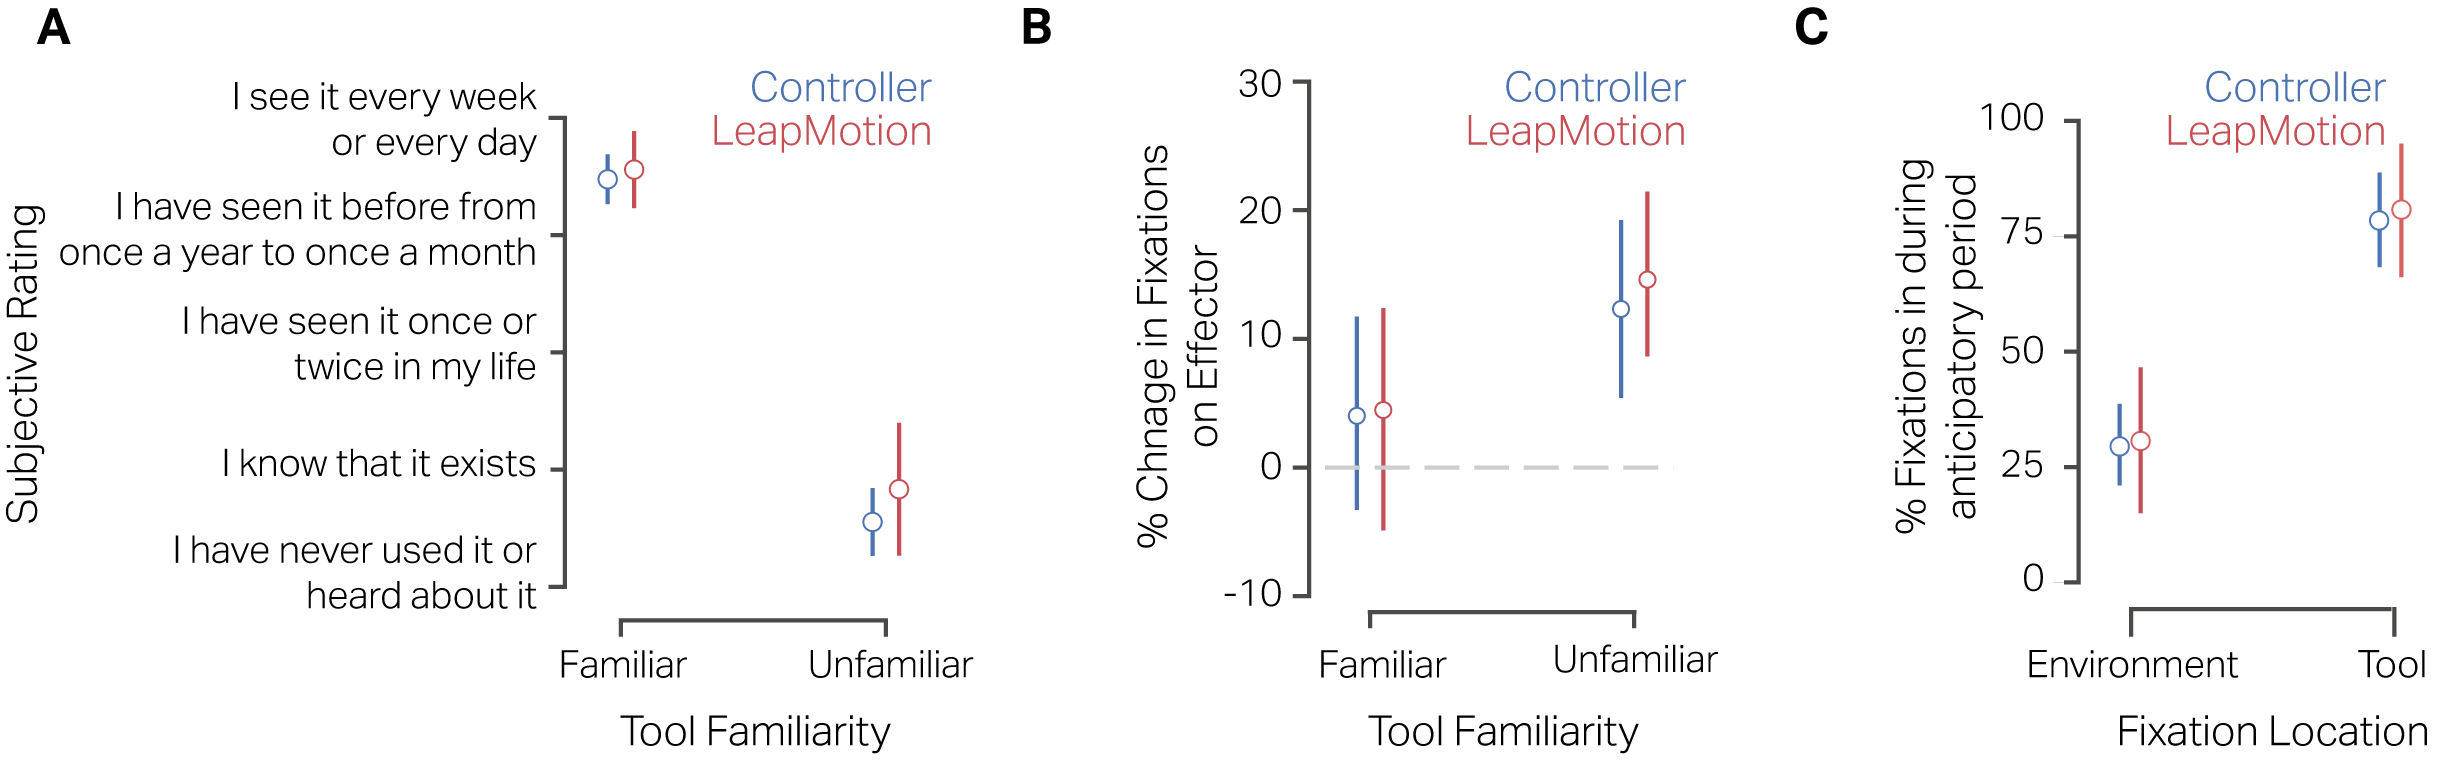
\includegraphics[width=1\linewidth]{source/figures/result/extra_analysis.png} \\
    \caption[]{ \textbf{A.}  Participants’ subjective rating of tool familiarity. Participants provided their subjective rating of familiarity with the 12 tool stimuli on a 5-point Likert-like scale. The circles correspond to the mean rating for each tool category, and error bars represent the standard deviation across subjects. \textbf{B.} Percentage change in fixations on the effector for the two different experiments. The circles correspond to the mean percentage change in across participants, and the error bars represent the standard error or mean. \textbf{C.} Percentage of fixations allocated to the environment vs. the tool during the 3s viewing period. The circles correspond to mean percentage of fixations across participants and the error denote the standard deviation.}
    \label{figure:familiarity_rating}
\end{figure}

Next, we analysed how the participants subjectively assessed the familiarity of the 12 tools and if there were any differences between the subjective ratings between the participants in experiment-I and II. \ref{figure:familiarity_rating}A shows the subjective familiarity ratings for each of the familiar and unfamiliar tools used in the study. The mean familiarity rating for familiar tools in experiment-I was 4.55 (SD=0.60) and for unfamiliar tools 1.81 (SD=1.17). In experiment-II, the mean familiarity rating for familiar tools was 4.48 (SD=0.52) and for unfamiliar tools 1.56 (SD=1.04). A mixed-ANOVA showed no differences in the familiarity ratings between the two experiments (F(1, 44)=3.08, p=0.06, $\eta_p^2 = 0.07$). Furthermore, there was a significant difference in the subjective rating of the tools (F(1, 44)=3094.05, p<0.001, $\eta_p^2=0.98$), i.e. the familiar tools were rated as subjectively familiar and the unfamiliar tools were rated subjectively unfamiliar. There were also no significant interactions between the two factors (F(1, 44)=2.52, p=0.11, $\eta_p^2=0.069$). In sum, our experimental condition of familiarity was consistent with the participants’ subjective rating as well. 

To determine if participants fixated on the tools' effector differently in later trials compared to earlier trials, we computed the percentage change of fixations on tool effector per tool familiarity. Figure \ref{figure:familiarity_rating}B shows the change in fixations on tool effector from first five and last five trials for familiar and unfamiliar tools in the two experiments. The mean percentage change in fixations on tool effector in experiment-I was 4.02 (SEM=7.27) for familiar tools and 12.32 (SEM=6.98) for unfamiliar tools. The mean percentage change in fixations allocated to tool effector in experiment-II was 4.47 (SEM=8.72) for familiar tools and 14.60 (SEM=6.32) for unfamiliar tools. The mixed-ANOVA showed no effect of the interaction methods on the percent change in fixations on tool effector (F(1, 46)=0.03, p=0.85, $\eta_p^2 = 0.0007$). There was also no effect of tool familiarity on percent change in fixations on the tool effector (F(1, 46)=1.26, p=0.26 $\eta_p^2 = 0.02$). There was also no interaction between the experiment groups and tool familiarity (F(1,46)=0.01, p=0.91 $\eta_p^2 = 0.0002$). Hence, we can conclude that participants did not allocate fixations differently on the tool effector in later trials compared to earlier trials.  

Lastly, we wanted to make sure that the differences in the virtual environments did not affect the way subjects allocated their attention to the experimental task. We calculated the percentage of fixations positioned on the tool vs. anywhere else in the environment for each subject across trials for the two experiments. Figure \ref{figure:familiarity_rating}C shows the percentage of fixations allocated to the tools vs. the environment for the two experiments during the 3s viewing period. For experiment-I with the interaction method of VR controller, the mean percentage of fixations on the environment was 0.29 (SD=0.06) and on the tools 0.80 (SD=0.09). Conversely, in experiment-II with LeapMotion as the interaction method, mean the percentage of fixations allocated to the environment was 0.30 (SD=0.15) and on the tools 0.80 (SD=0.14). The mixed-ANOVA showed no differences in the percentage of fixations between the two experiments (F(1, 47)=2.86, p=0.09, $\eta_p^2=0.05$). There were significant differences in the percentage of fixations located on the tool vs. the environment (F(1, 47)=217.47, p<0.001, $\eta_p^2=0.82$). We did not find any interactions between the two factors (F(1, 47)=0.02, p=0.87, $\eta_p^2=0.0004$). These results show that fixations were primarily made in a task-oriented manner and were not affected by the differences in the virtual environment of the two experiments.



